%%%%%%%%%%%%%%%%%%%%%%%%%%%%%%%%%%%%%%%%%%%%%%%%%%%%%%%%%%%%%%%%%%%%%%%%
% A0 Academic Poster — Deep Hedging Research
% Author: Pratham Kailasiya, IIT Roorkee
% Framework: tikzposter | Size: 33in x 46in (A0 Portrait)
% Layout: 2-column, 4-row grid with 8 content sections + footer
%%%%%%%%%%%%%%%%%%%%%%%%%%%%%%%%%%%%%%%%%%%%%%%%%%%%%%%%%%%%%%%%%%%%%%%%
\documentclass[25pt, a0paper, portrait]{tikzposter}

%% ─── Packages ───────────────────────────────────────────────────────
\usepackage[utf8]{inputenc}
\usepackage[T1]{fontenc}
\usepackage{helvet}
\renewcommand{\familydefault}{\sfdefault}
\usepackage{amsmath,amssymb,amsthm}
\usepackage{mathtools}
\usepackage{booktabs}
\usepackage{enumitem}
\usepackage{graphicx}
\usepackage{pifont}
\usepackage{xcolor}
\usepackage{tikz}
\usetikzlibrary{shapes.geometric,arrows.meta,positioning,fit,calc,
                 decorations.pathreplacing,backgrounds}
\usepackage{multicol}
\usepackage{tabularx}

%% ─── Figure path ────────────────────────────────────────────────────
\graphicspath{{poster_figs/}}

%% ─── Math shortcuts ─────────────────────────────────────────────────
\newcommand{\E}{\mathbb{E}}
\newcommand{\R}{\mathbb{R}}
\newcommand{\PP}{\mathbb{P}}
\newcommand{\QQ}{\mathbb{Q}}
\newcommand{\cvar}{\mathrm{CVaR}}
\newcommand{\VaR}{\mathrm{VaR}}
\DeclareMathOperator*{\argmin}{arg\,min}

%% ═══════════════════════════════════════════════════════════════════
%% COLOR PALETTE — Inspired by reference poster (teal/blue academic)
%% ═══════════════════════════════════════════════════════════════════
\definecolor{PosterBG}{HTML}{FFFFFF}
\definecolor{BlockBG}{HTML}{FFFFFF}
\definecolor{HeaderBG}{HTML}{0E7490}      % Teal primary
\definecolor{NavyPri}{HTML}{164E63}       % Dark teal for headings
\definecolor{SoftBlue}{HTML}{0891B2}      % Lighter teal accent
\definecolor{AccWarm}{HTML}{D97706}       % Warm amber accent
\definecolor{AccGreen}{HTML}{059669}      % Green accent
\definecolor{LightBG}{HTML}{F0FDFA}       % Teal tinted light bg
\definecolor{TextDark}{HTML}{1E293B}      % Near-black body
\definecolor{TextBody}{HTML}{334155}      % Slate body text
\definecolor{RuleGray}{HTML}{CBD5E1}      % Subtle rule color
\definecolor{GreenOK}{HTML}{16A34A}       % Checkmark green
\definecolor{NumCircle}{HTML}{0E7490}     % Section number circles

%% ─── tikzposter theme ───────────────────────────────────────────────
\definecolorstyle{TealAcademic}{
  \colorlet{colorOne}{HeaderBG}
  \colorlet{colorTwo}{SoftBlue}
  \colorlet{colorThree}{BlockBG}
}{
  \colorlet{blocktitlebgcolor}{NavyPri}
  \colorlet{blocktitlefgcolor}{white}
  \colorlet{blockbodybgcolor}{BlockBG}
  \colorlet{blockbodyfgcolor}{TextBody}
  \colorlet{backgroundcolor}{PosterBG}
  \colorlet{framecolor}{PosterBG}
}

\usetheme{Default}
\usecolorstyle{TealAcademic}
\useblockstyle[roundedcorners=8]{Default}
\usetitlestyle{Default}

%% ─── Numbered section command ───────────────────────────────────────
\newcommand{\secnum}[1]{%
  \tikz[baseline=(n.base)]{\node[circle,fill=NumCircle,text=white,
  inner sep=3pt,font=\bfseries\Large] (n) {#1};}%
}

%% ─── Equation highlight box ────────────────────────────────────────
\newcommand{\eqbox}[1]{%
  \colorbox{LightBG}{\parbox{0.93\linewidth}{\vspace{4pt}#1\vspace{4pt}}}%
}

%% ═══════════════════════════════════════════════════════════════════
%% TITLE / HEADER
%% ═══════════════════════════════════════════════════════════════════
\title{\parbox{0.97\linewidth}{%
  \begin{minipage}[c]{0.10\linewidth}
    
\includegraphics[height=7.5cm]{iitr_logo.png}
  \end{minipage}%
  \hfill
  \begin{minipage}[c]{0.87\linewidth}
    \centering
    {\fontsize{70}{84}\selectfont\bfseries\color{white}%
    Computational and Deep Learning Strategies\\[4pt]
    in Quantitative Finance for Robust Hedging\\[4pt]
    under Market Frictions}\\[12pt]
    {\fontsize{32}{38}\selectfont\color{white!90}%
    MA-500B Thesis Mid Semester Evaluation}
  \end{minipage}%
}}

\author{%
  {\fontsize{36}{42}\selectfont\bfseries\color{white} Pratham Kailasiya}%
  \quad{\fontsize{28}{34}\selectfont\color{white!85}%
  Enrollment No.\ 21323030%
  \quad$\boldsymbol{\cdot}$\quad%
  BS-MS, Mathematics and Computing%
  \quad$\boldsymbol{\cdot}$\quad%
  Minor: Business Management Studies}\\[6pt]%
  {\fontsize{28}{34}\selectfont\color{white!85}%
  Supervisor: \textbf{Prof.\ Aditi Gangopadhyay}%
  \quad$\boldsymbol{\cdot}$\quad%
  Department of Mathematics%
  \quad$\boldsymbol{\cdot}$\quad%
  Indian Institute of Technology Roorkee}%
}
\institute{}

%% ═══════════════════════════════════════════════════════════════════
\begin{document}

\maketitle[width=0.97\textwidth, titletotopverticalspace=8mm,
           titletoblockverticalspace=18mm]

%% ═════════════════════ ROW 1 ═════════════════════════════════════
\begin{columns}

%% ── SECTION 1: Introduction & Motivation ─────────────────────────
\column{0.48}
\block{\secnum{1}\;\; Introduction \& Motivation}{
\color{TextBody}
Classical Black--Scholes delta hedging assumes known dynamics, continuous
rebalancing, and zero transaction costs---all violated in practice.
\textbf{Deep hedging} (Buehler et al., 2019) learns strategies directly
from simulated paths, but three \textbf{critical gaps} remain:

\bigskip
\begin{center}
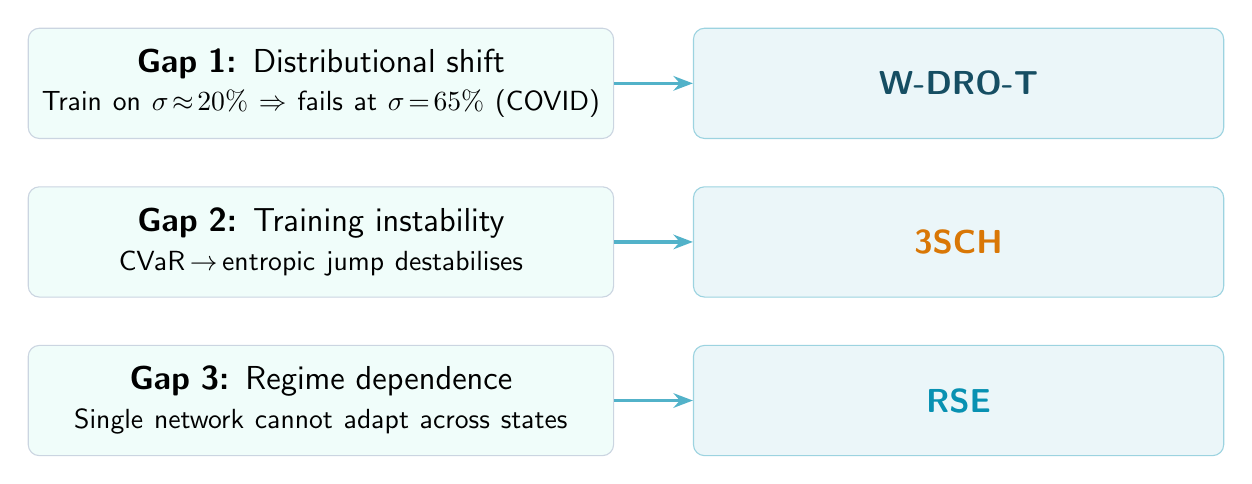
\begin{tikzpicture}[
  gap/.style={rectangle,rounded corners=4pt,draw=RuleGray,fill=LightBG,
              minimum height=14mm,text width=7.2cm,text centered,
              font=\large},
  sol/.style={rectangle,rounded corners=4pt,draw=SoftBlue!40,
              fill=SoftBlue!8,minimum height=14mm,text width=6.5cm,
              text centered,font=\large\bfseries},
  arr/.style={-{Stealth[length=7pt]},very thick,SoftBlue!70}]
\node[gap] (g1) {\textbf{Gap 1:} Distributional shift\\
  {\normalsize Train on $\sigma\!\approx\!20\%$ $\Rightarrow$
   fails at $\sigma\!=\!65\%$ (COVID)}};
\node[gap,below=6mm of g1] (g2) {\textbf{Gap 2:} Training instability\\
  {\normalsize CVaR\,$\to$\,entropic jump destabilises}};
\node[gap,below=6mm of g2] (g3) {\textbf{Gap 3:} Regime dependence\\
  {\normalsize Single network cannot adapt across states}};
\node[sol,right=10mm of g1] (s1) {\color{NavyPri}W-DRO-T};
\node[sol,right=10mm of g2] (s2) {\color{AccWarm}3SCH};
\node[sol,right=10mm of g3] (s3) {\color{SoftBlue}RSE};
\draw[arr] (g1) -- (s1);
\draw[arr] (g2) -- (s2);
\draw[arr] (g3) -- (s3);
\end{tikzpicture}
\end{center}

\bigskip
\textbf{Three novel approaches} proposed in this work:
\begin{itemize}[leftmargin=1.2em,itemsep=3pt,labelsep=0.4em,topsep=4pt]
\item[$\triangleright$] \textbf{W-DRO-T:} Wasserstein DRO Transformer ---
  distributional robustness via gradient penalty
\item[$\triangleright$] \textbf{3SCH:} Three-Stage Curriculum Hedger ---
  smooth homotopy from CVaR to entropic risk
\item[$\triangleright$] \textbf{RSE:} Regime-Switching Ensemble ---
  soft gating across LSTM, Transformer, Signature models
\end{itemize}

\medskip
\textbf{Experimental protocol:}\;
80\,K Heston paths $\cdot$ $N\!=\!30$ steps $\cdot$ 10 seeds
$\cdot$ 10\,K bootstrap $\cdot$ Holm--Bonferroni correction
$\cdot$ Cohen's $d$ effect sizes $\cdot$ Real-market validation
on \textbf{SPY} and \textbf{NIFTY\,50} under normal, COVID-19,
and GFC-2008 regimes.
}

%% ── SECTION 2: Mathematical Framework ────────────────────────────
\column{0.48}
\block{\secnum{2}\;\; Mathematical Framework}{
\color{TextBody}

\textbf{\color{NavyPri}Heston stochastic-volatility model}

\eqbox{
\begin{align*}
dS_t &= rS_t\,dt + \sqrt{v_t}\,S_t\,dW^S_t, \\
dv_t &= \kappa(\theta_v - v_t)\,dt + \xi\sqrt{v_t}\,dW^v_t,
\quad dW^S \!\cdot\! dW^v = \rho\,dt
\end{align*}
}

\smallskip
Parameters: $S_0\!=\!K\!=\!100$, $v_0\!=\!\theta_v\!=\!0.04$,
$\kappa\!=\!1.0$, $\xi\!=\!0.2$, $\rho\!=\!{-}0.7$, $r\!=\!0.05$.
Euler--Maruyama full-truncation discretisation, $N\!=\!30$ daily steps.

\bigskip
\textbf{\color{NavyPri}Deep hedging P\&L and objective}

\eqbox{
\vspace{-8pt}
\[
\Pi(\delta) = -Z + \sum_{k=0}^{N-1} \delta_k (S_{t_{k+1}} - S_{t_k})
  - c_{\mathrm{tc}}\sum_{k=0}^{N} |\delta_k - \delta_{k-1}| S_{t_k}
\]
\vspace{-8pt}
}

\smallskip
with $c_{\mathrm{tc}}\!=\!0.001$, $Z\!=\!\max(S_T\!-\!K,0)$,
$\delta_k \in [-1.5, 1.5]$.

\bigskip
\textbf{\color{NavyPri}Risk measures}

\begin{minipage}[t]{0.48\linewidth}
\textbf{CVaR (tail-focused):}
\vspace{-4pt}
\[
\cvar_\alpha(L) = \inf_\nu\Bigl\{\nu + \frac{\E[(L-\nu)^+]}{1-\alpha}\Bigr\}
\]
\end{minipage}
\hfill
\begin{minipage}[t]{0.48\linewidth}
\textbf{Entropic (global):}
\vspace{-4pt}
\[
\rho_\lambda(X) = \frac{1}{\lambda}\log\E[\exp(-\lambda X)]
\]
\end{minipage}

\bigskip
\begin{center}
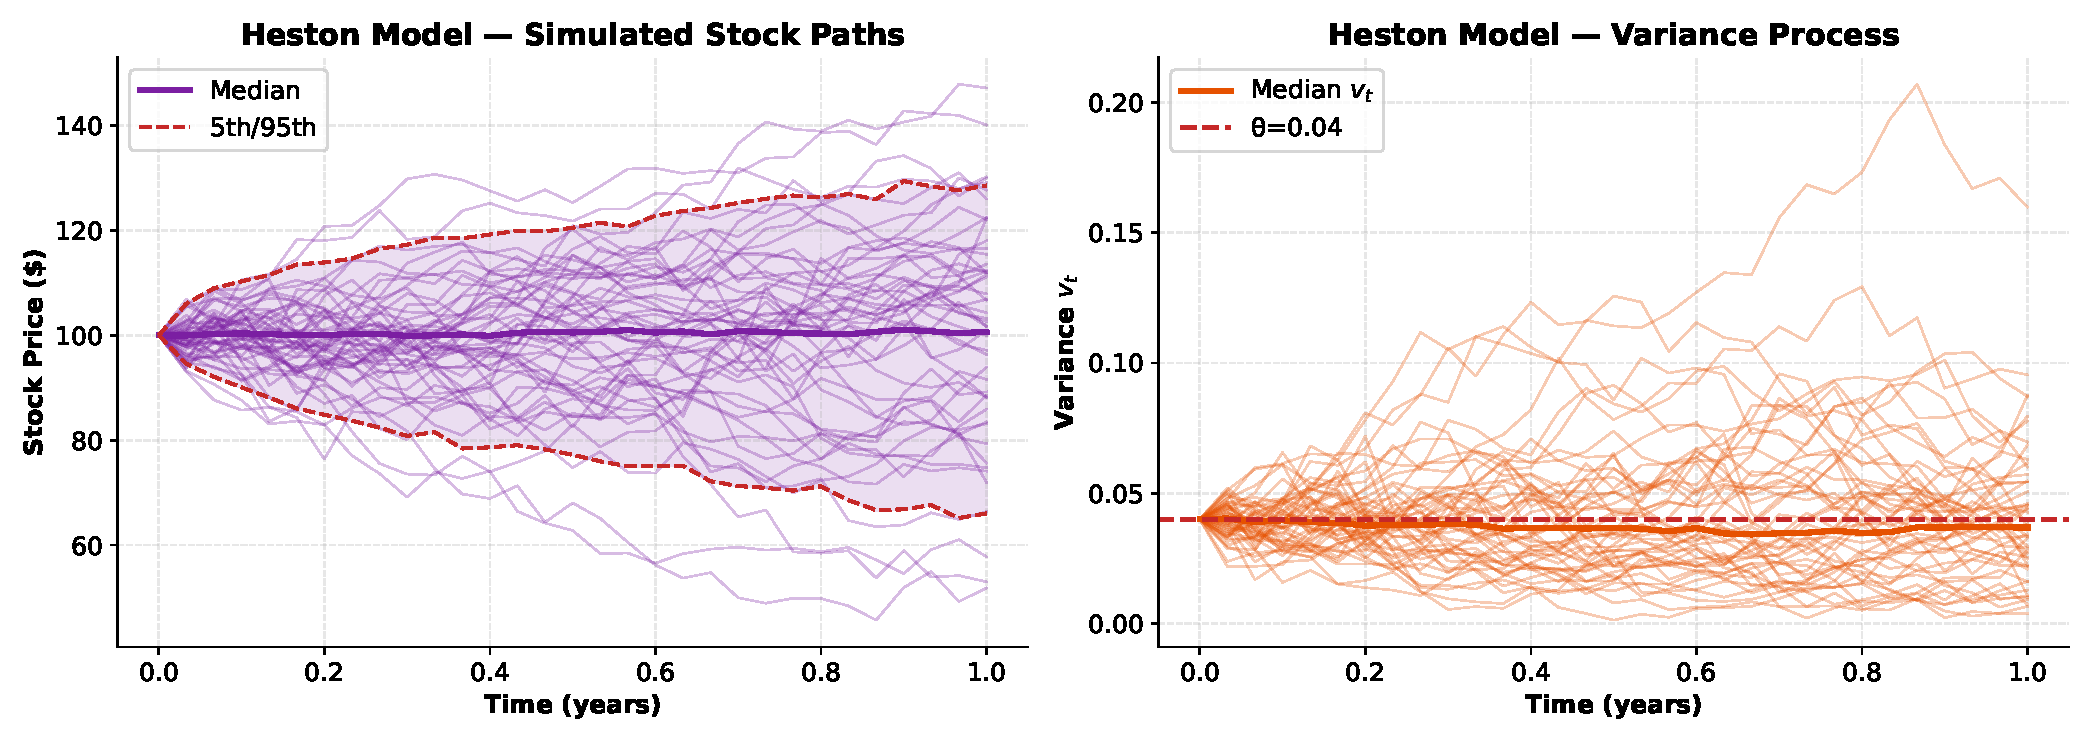
\includegraphics[width=0.92\linewidth]{heston_paths.pdf}
\end{center}
\vspace{-4pt}
{\small\color{NavyPri}\textbf{Figure:} Simulated Heston stock price paths
(left) and stochastic variance process (right).}
}

\end{columns}

%% ═════════════════════ ROW 2 ═════════════════════════════════════
\begin{columns}

%% ── SECTION 3: Proposed Methods ──────────────────────────────────
\column{0.48}
\block{\secnum{3}\;\; Hedging Architectures \& Proposed Methods}{
\color{TextBody}

%% --- W-DRO-T ---
\textbf{\Large\color{NavyPri}Wasserstein DRO Transformer (W-DRO-T)}

\smallskip
Minimises worst-case risk over a Wasserstein ambiguity set.
Via Kantorovich duality, the intractable inner supremum reduces to
a \textbf{gradient-norm penalty}:

\eqbox{
\vspace{-6pt}
\[
\mathcal{L}_{\mathrm{DRO}}(\theta)
  = \E_\PP[\ell(\theta;X)]
  + \varepsilon\,\E_\PP\!\bigl[\|\nabla_{\!X}\ell(\theta;X)\|_2\bigr],
  \quad \varepsilon\!:\; 0 \!\to\! 0.1
\]
\vspace{-6pt}
}

\smallskip
\begin{itemize}[leftmargin=1em,itemsep=2pt,labelsep=0.3em,topsep=2pt]
\item[$\triangleright$] Transformer encoder with causal mask (non-anticipativity)
\item[$\triangleright$] 2\textsuperscript{nd}-order gradients via
      \texttt{create\_graph=True}; forces MATH SDPA backend
\item[$\triangleright$] 3-phase: CVaR pretrain (50\,ep)
      $\to$ DRO-annealed entropic (30\,ep) $\to$ stress test (10\,ep)
\item[$\triangleright$] Architecture: $d_{\mathrm{model}}\!=\!64$,
      $H\!=\!4$, $L\!=\!3$, $\sim$85K params, $\sim$7\,119\,s/seed
\end{itemize}

\bigskip
%% --- 3SCH ---
\textbf{\Large\color{AccWarm}Three-Stage Curriculum Hedger (3SCH)}

\smallskip
Smooth homotopy from CVaR to entropic via mixed loss:

\eqbox{
\vspace{-6pt}
\[
\mathcal{L}_{\mathrm{mix}}(\alpha;\theta)
  = \alpha\,\cvar_{0.95}(-\Pi^\theta)
  + (1\!-\!\alpha)\,\rho_\lambda(-\Pi^\theta),
  \quad \alpha\!:\; 0.8 \!\to\! 0.2
\]
\vspace{-6pt}
}

\smallskip
\begin{itemize}[leftmargin=1em,itemsep=2pt,labelsep=0.3em,topsep=2pt]
\item[$\triangleright$] Stage 1: CVaR pretrain (50\,ep)
      $\to$ Stage 2: $\alpha$-anneal (20\,ep)
      $\to$ Stage 3: entropic fine-tune (30\,ep)
\item[$\triangleright$] \textbf{Same} LSTM architecture as baseline ($\sim$54K params)
      --- novelty is \emph{purely} in the training schedule
\item[$\triangleright$] Zero-cost rollback: set $T_2\!=\!0$ to recover
      two-stage baseline
\end{itemize}

\bigskip
%% --- RSE ---
\textbf{\Large\color{SoftBlue}Regime-Switching Ensemble (RSE)}

\smallskip
Soft gating of LSTM, Transformer, and Signature hedgers via
learned regime--model affinity:

\eqbox{
\vspace{-6pt}
\[
\delta_k^{\mathrm{RSE}} = \sum_{m=1}^{3} w_m(r_k)\,\delta_k^{(m)},
\quad
w_m = \sum_{j=1}^{K} p(r_k\!=\!j)\,[\mathrm{softmax}(A/\tau)]_{jm}
\]
\vspace{-6pt}
}

\smallskip
\begin{itemize}[leftmargin=1em,itemsep=2pt,labelsep=0.3em,topsep=2pt]
\item[$\triangleright$] 6 regime features: RV$^{(5,10,20)}$, trend, momentum,
      jump (Barndorff-Nielsen bipower)
\item[$\triangleright$] $K\!=\!4$ regimes: calm, stressed, trending,
      mean-reverting
\item[$\triangleright$] Affinity $A \in \R^{4\times 3}$:
      LSTM dominates calm; Transformer dominates stressed
\end{itemize}

\medskip
\begin{center}
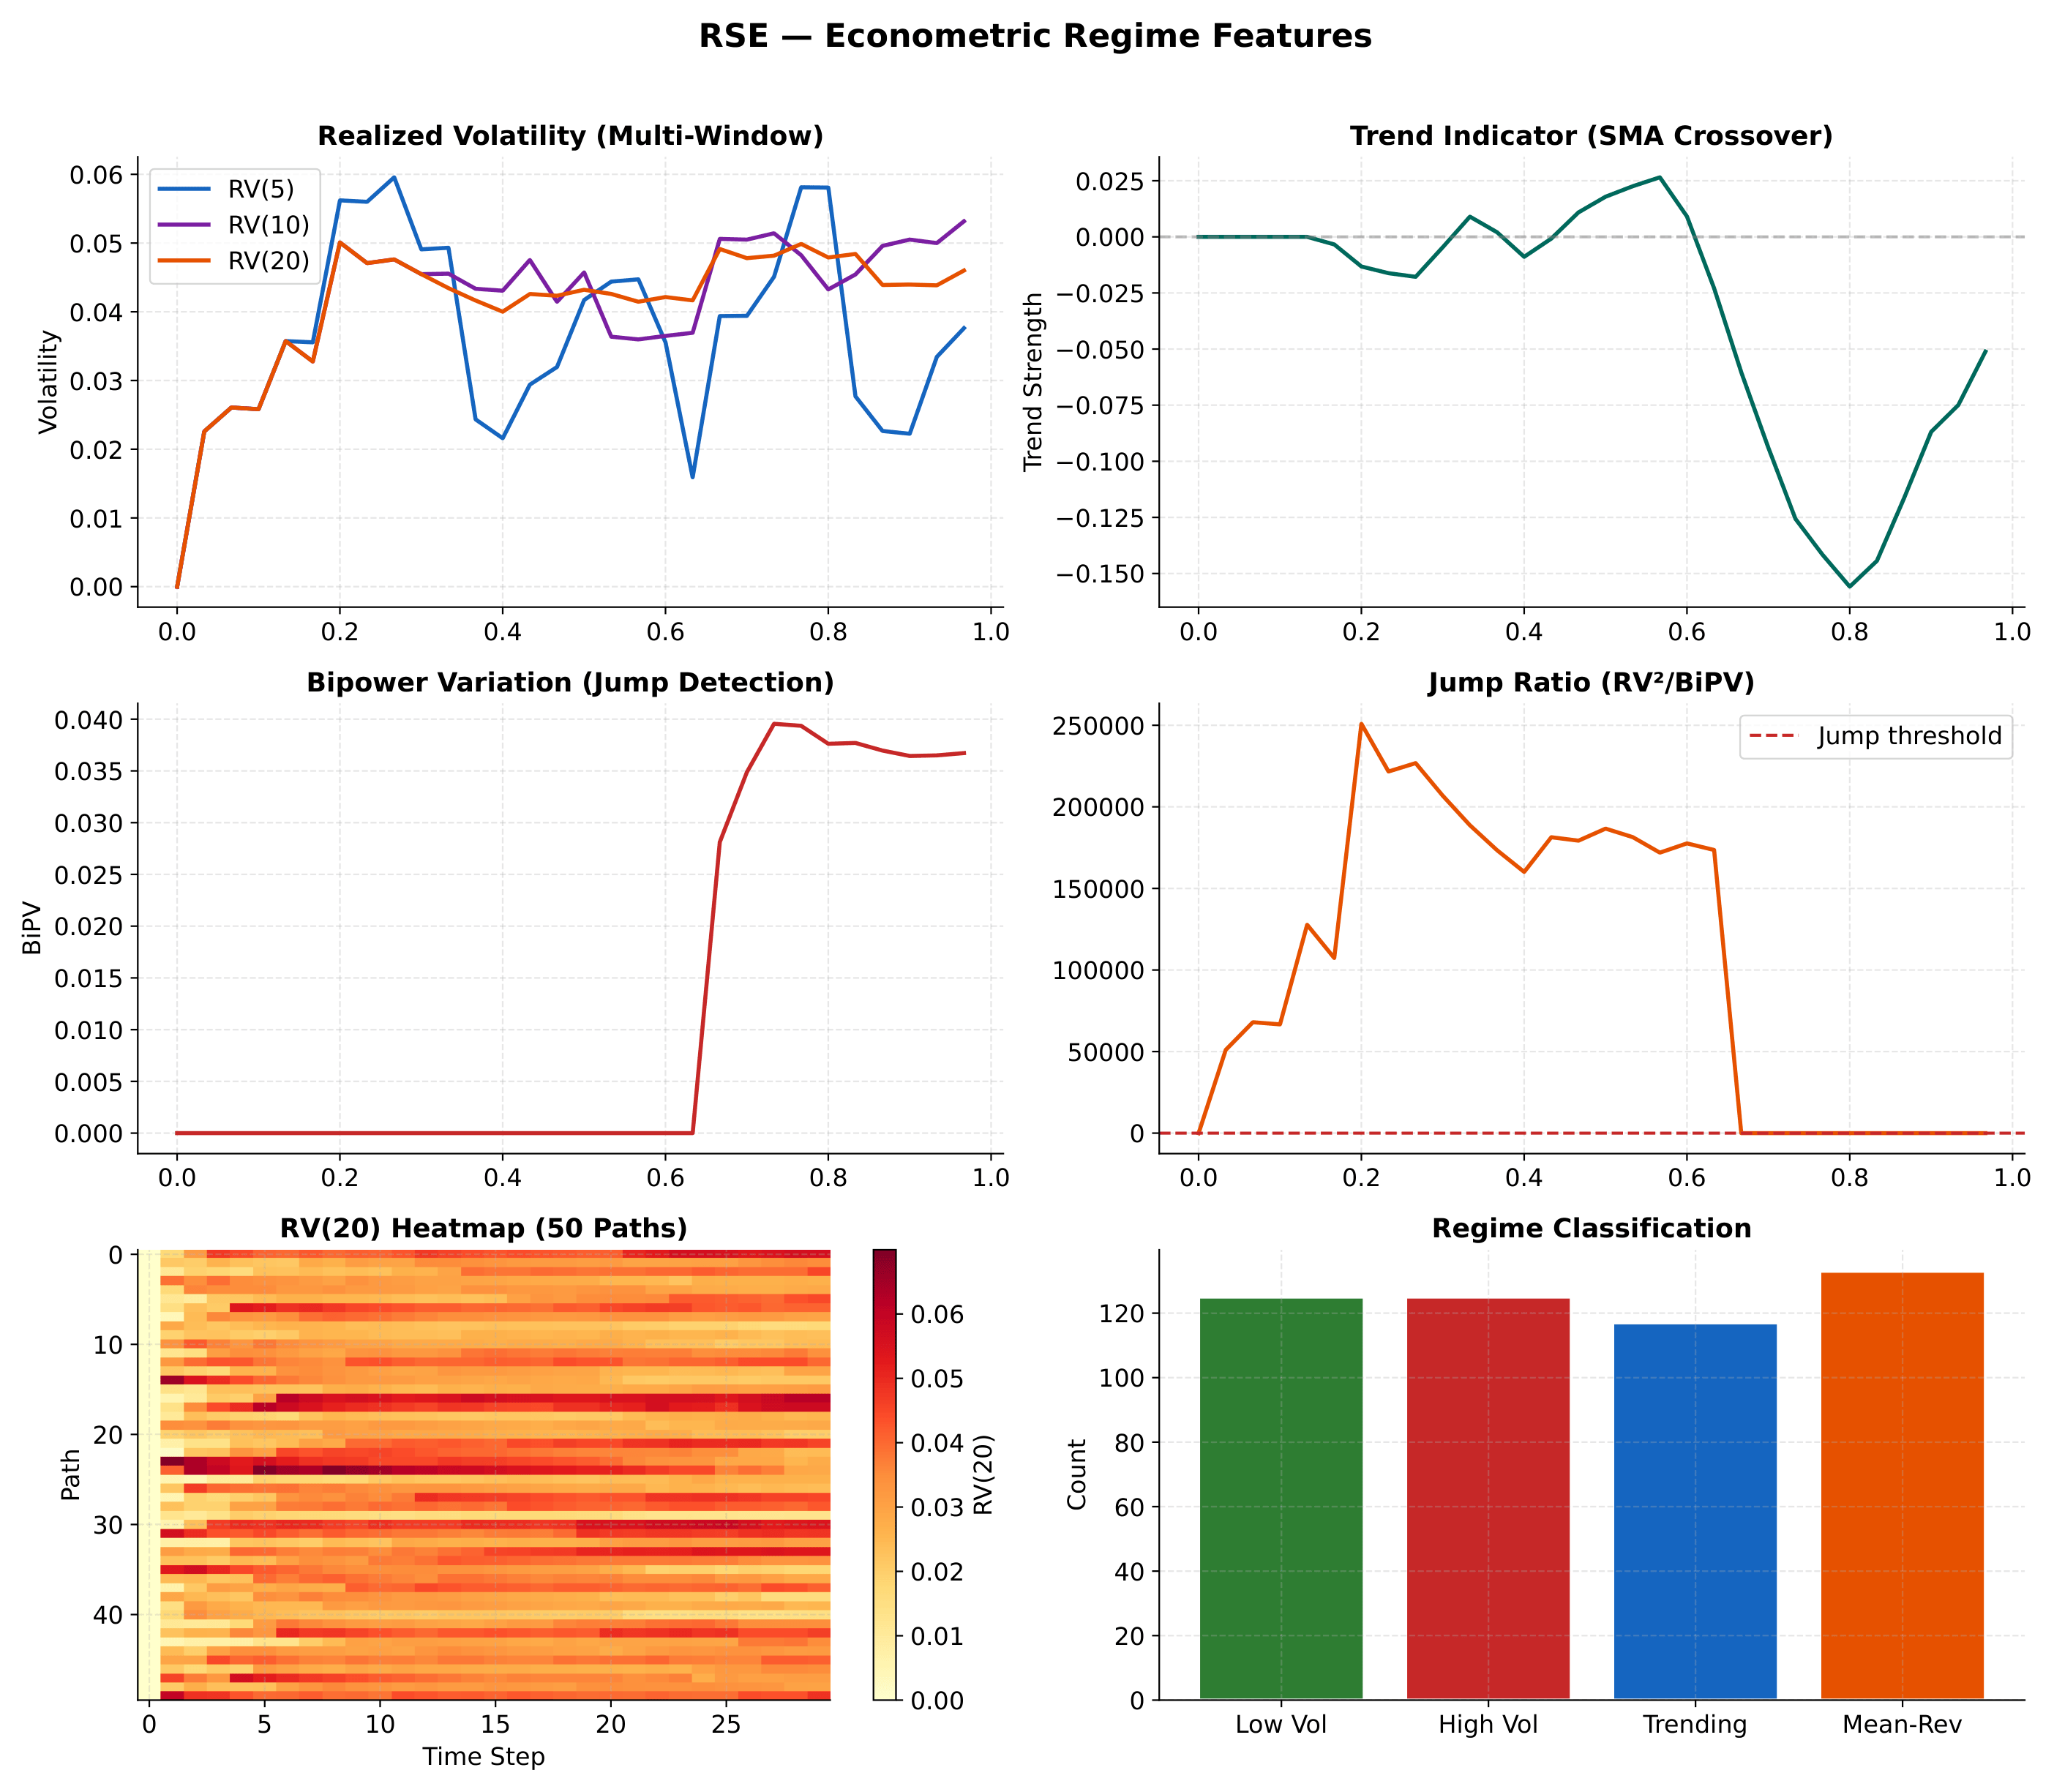
\includegraphics[width=0.92\linewidth]{rse_regime_features.png}
\end{center}
\vspace{-4pt}
{\small\color{NavyPri}\textbf{Figure:} RSE econometric regime feature
extraction pipeline.}
}

%% ── SECTION 4: Experimental Results ──────────────────────────────
\column{0.48}
\block{\secnum{4}\;\; Experimental Results}{
\color{TextBody}

\textbf{\color{NavyPri}Main performance (10 seeds, 50K train paths)}

\medskip
\renewcommand{\arraystretch}{1.25}
\setlength{\tabcolsep}{5pt}
{\normalsize
\begin{tabular}{@{}l c c c c c@{}}
\toprule
\textbf{Model} & \textbf{CVaR$_{95}$} & \textbf{Std}
  & \textbf{Entropic} & \textbf{Vol.} & \textbf{CV\%} \\
\cmidrule(r){1-1}\cmidrule(lr){2-2}\cmidrule(lr){3-3}
\cmidrule(lr){4-4}\cmidrule(lr){5-5}\cmidrule(l){6-6}
\textbf{RSE}    & $\mathbf{3.109\!\pm\!0.010}$ & 0.456 & 2.376 & 1.379
  & \textbf{0.30} \\
LSTM             & $3.215\!\pm\!0.018$ & 0.449 & 2.379 & 1.137 & 0.55 \\
3SCH             & $3.219\!\pm\!0.022$ & 0.453 & 2.381 & 1.122 & 0.69 \\
W-DRO-T          & $3.227\!\pm\!0.024$ & 0.450 & 2.380 & 1.119 & 0.75 \\
Transformer      & $3.234\!\pm\!0.030$ & 0.450 & 2.380 & 1.117 & 0.92 \\
\bottomrule
\end{tabular}}

\medskip
{\small\color{NavyPri} Lower is better for all metrics. RSE achieves
\textbf{best CVaR$_{95}$} and \textbf{lowest CV\%} (most stable).}

\bigskip
\textbf{\color{NavyPri}Statistical comparison vs.\ LSTM baseline}

\medskip
{\normalsize
\begin{tabular}{@{}l c c c@{}}
\toprule
\textbf{Model} & \textbf{95\% Bootstrap CI} & \textbf{$p$-value}
  & \textbf{Cohen's $d$} \\
\cmidrule(r){1-1}\cmidrule(lr){2-2}\cmidrule(lr){3-3}\cmidrule(l){4-4}
RSE     & $[3.104,\; 3.115]$ & $<\!0.0001^{***}$ & $-7.41$ (huge) \\
3SCH    & $[3.210,\; 3.229]$ & $0.58$             & $+0.19$ (neg.)  \\
W-DRO-T & $[3.220,\; 3.234]$ & $0.10$             & $+0.60$ (med.)  \\
\bottomrule
\end{tabular}}

\medskip
{\small\color{NavyPri} RSE is the only model with statistically significant
improvement over LSTM ($p\!<\!0.0001$, $|d|\!=\!7.41$).
All CIs via 10\,000 bootstrap resamples; Holm--Bonferroni corrected.}

\bigskip
\begin{center}
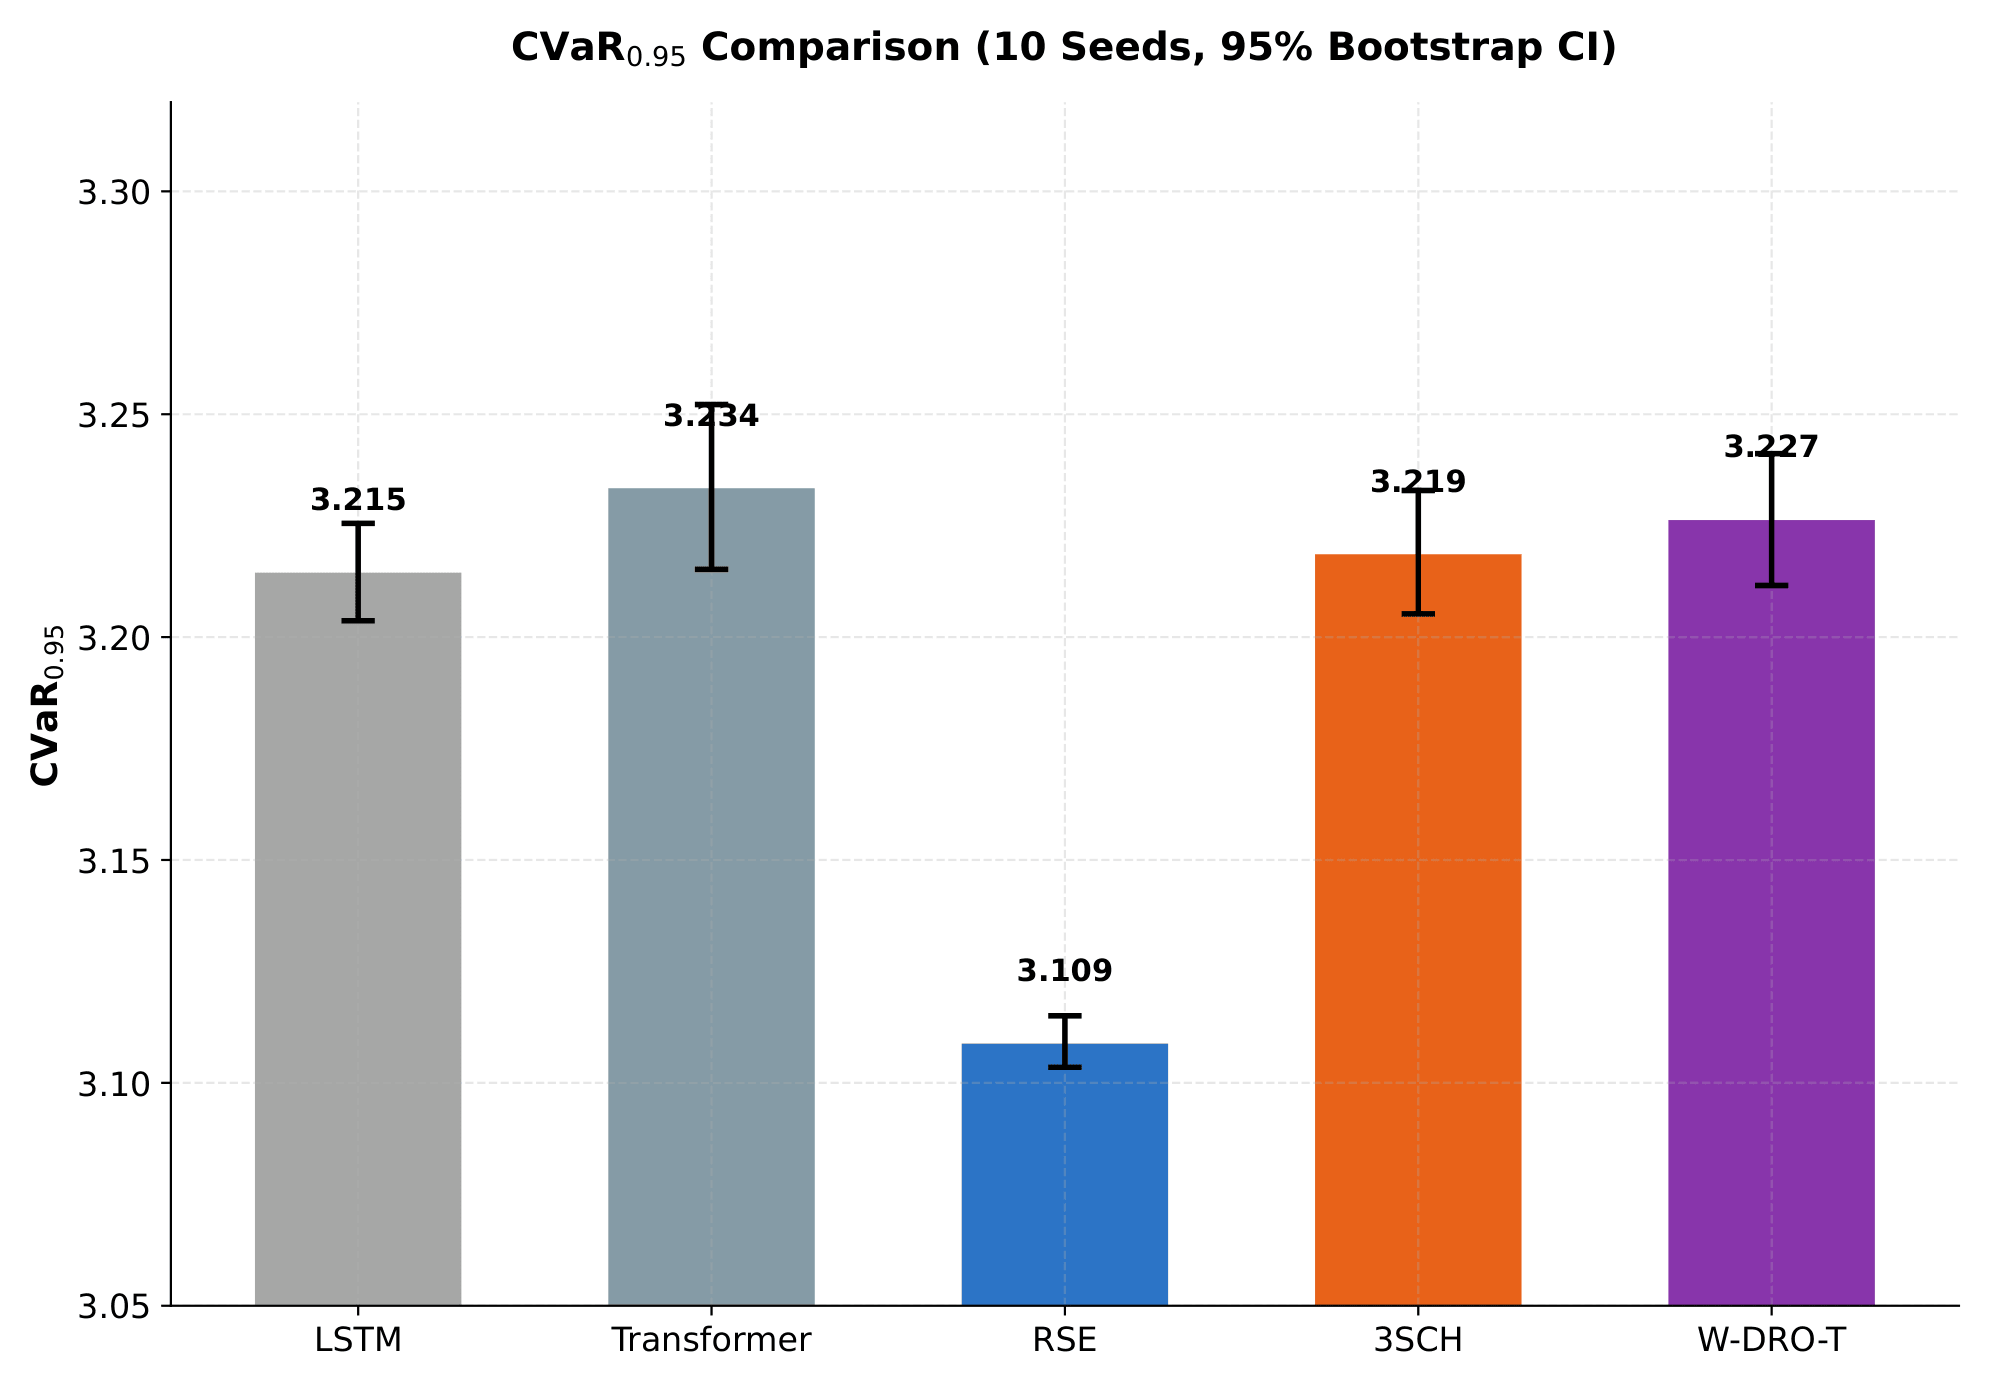
\includegraphics[width=0.92\linewidth]{cvar_bootstrap.png}
\end{center}
\vspace{-4pt}
{\small\color{NavyPri}\textbf{Figure:} CVaR$_{0.95}$ comparison with
95\% bootstrap confidence intervals across all models.}

\bigskip
\begin{center}
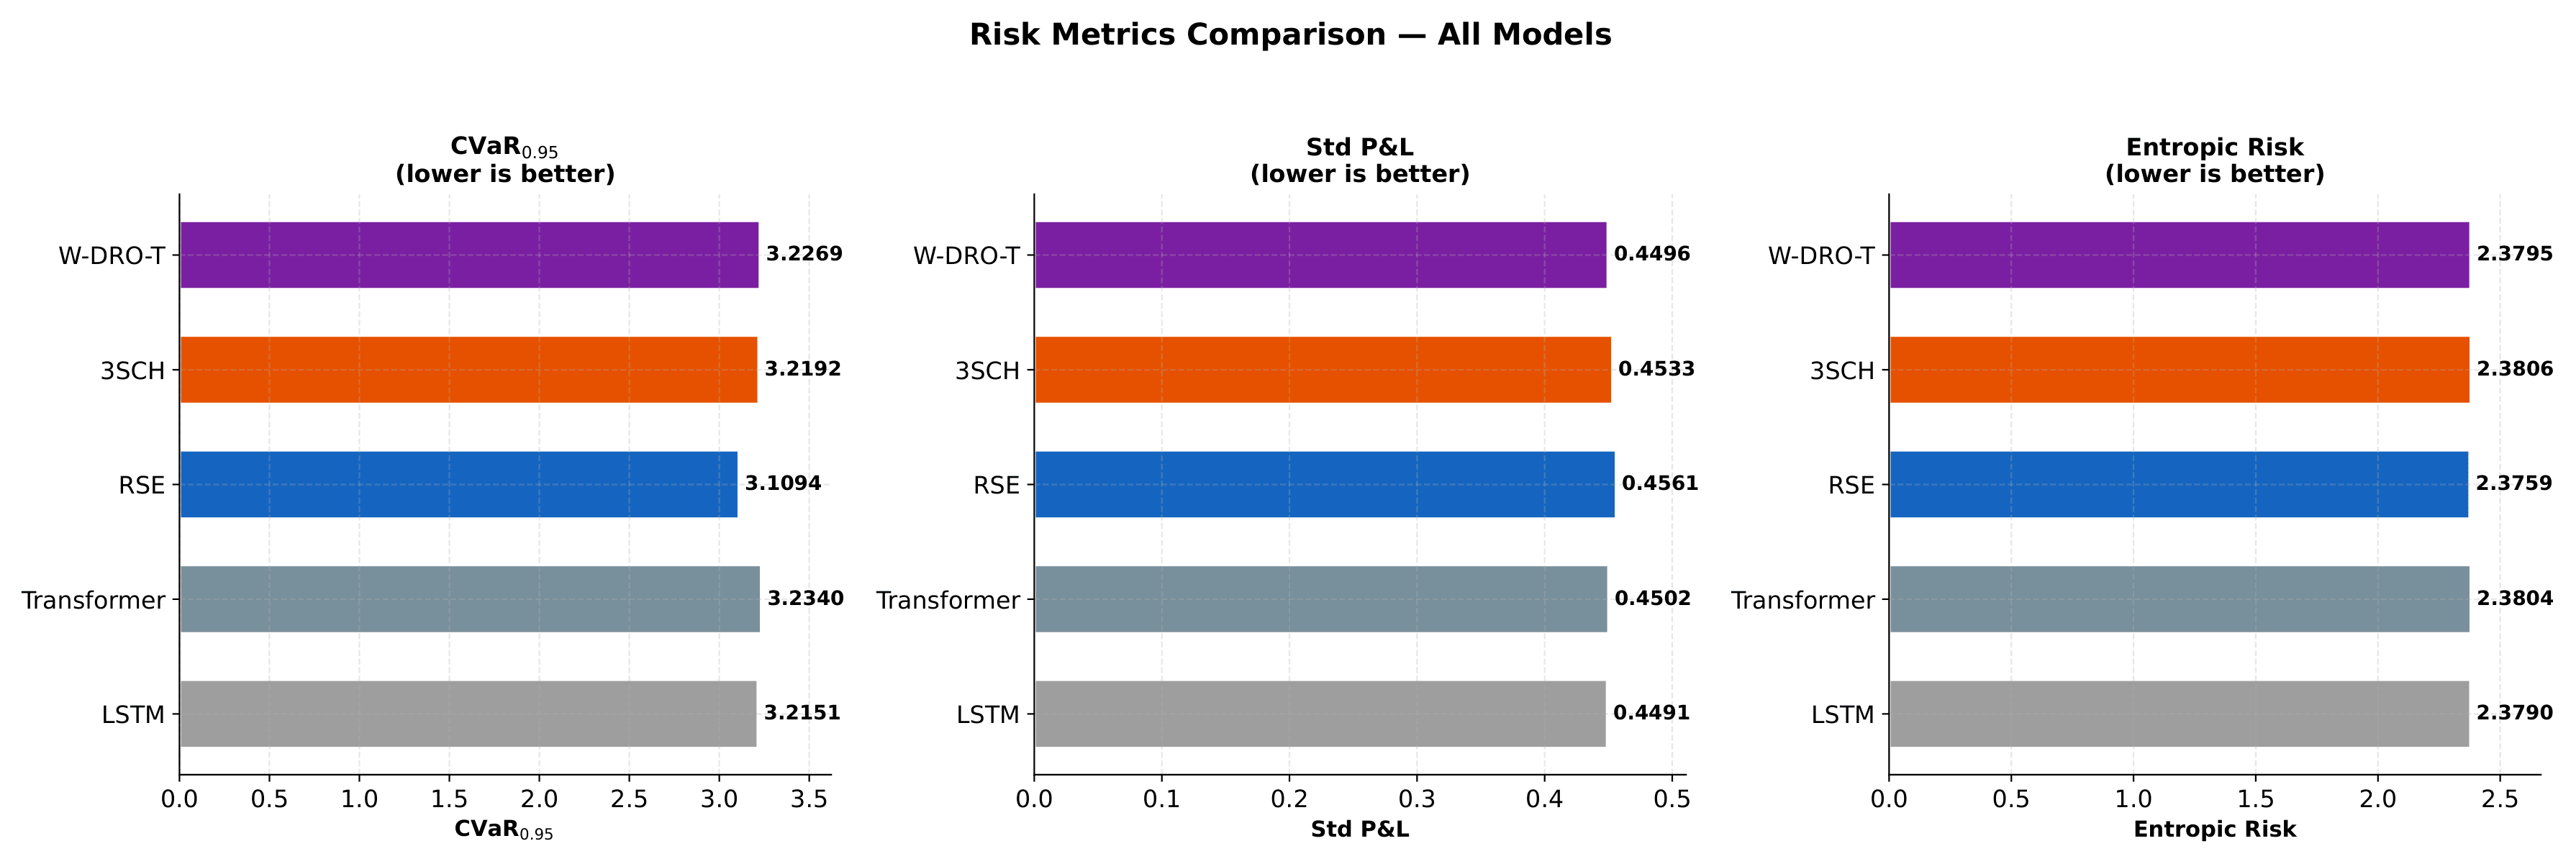
\includegraphics[width=0.92\linewidth]{risk_metrics_comparison.png}
\end{center}
\vspace{-4pt}
{\small\color{NavyPri}\textbf{Figure:} Multi-metric risk comparison
across all models (CVaR, Entropic, Std P\&L).}
}

\end{columns}

%% ═════════════════════ ROW 3 ═════════════════════════════════════
\begin{columns}

%% ── SECTION 5: Real Market Validation & Crisis Testing ───────────
\column{0.48}
\block{\secnum{5}\;\; Real Market Validation \& Crisis Testing}{
\color{TextBody}

Heston parameters calibrated to historical SPY and NIFTY\,50 data
across \textbf{three regimes}: Normal (2019--2020 pre-COVID),
COVID-19 ($\sigma\!\approx\!65\%$), and GFC-2008 ($\sigma\!\approx\!80\%$).

\bigskip
\textbf{\color{NavyPri}SPY (US Market, $\sim$5\,bps cost)}

\medskip
{\normalsize
\begin{tabular}{@{}l c c c@{}}
\toprule
\textbf{Model} & \textbf{Normal} & \textbf{COVID-19} & \textbf{GFC-2008} \\
\cmidrule(r){1-1}\cmidrule(lr){2-2}\cmidrule(lr){3-3}\cmidrule(l){4-4}
\textbf{W-DRO-T} & \textbf{11.98} & \textbf{46.94} & \textbf{62.26} \\
Transformer       & 14.47          & 60.09          & 80.19 \\
3SCH              & 15.79          & 69.25          & 88.43 \\
RSE               & 16.90          & 69.76          & 84.57 \\
LSTM              & 20.28          & 86.84          & 100.88 \\
\bottomrule
\end{tabular}}

\medskip
{\small W-DRO-T dominates all SPY scenarios: $-41\%$ (normal),
$-46\%$ (COVID), $-38\%$ (GFC) vs LSTM.}

\bigskip
\begin{center}
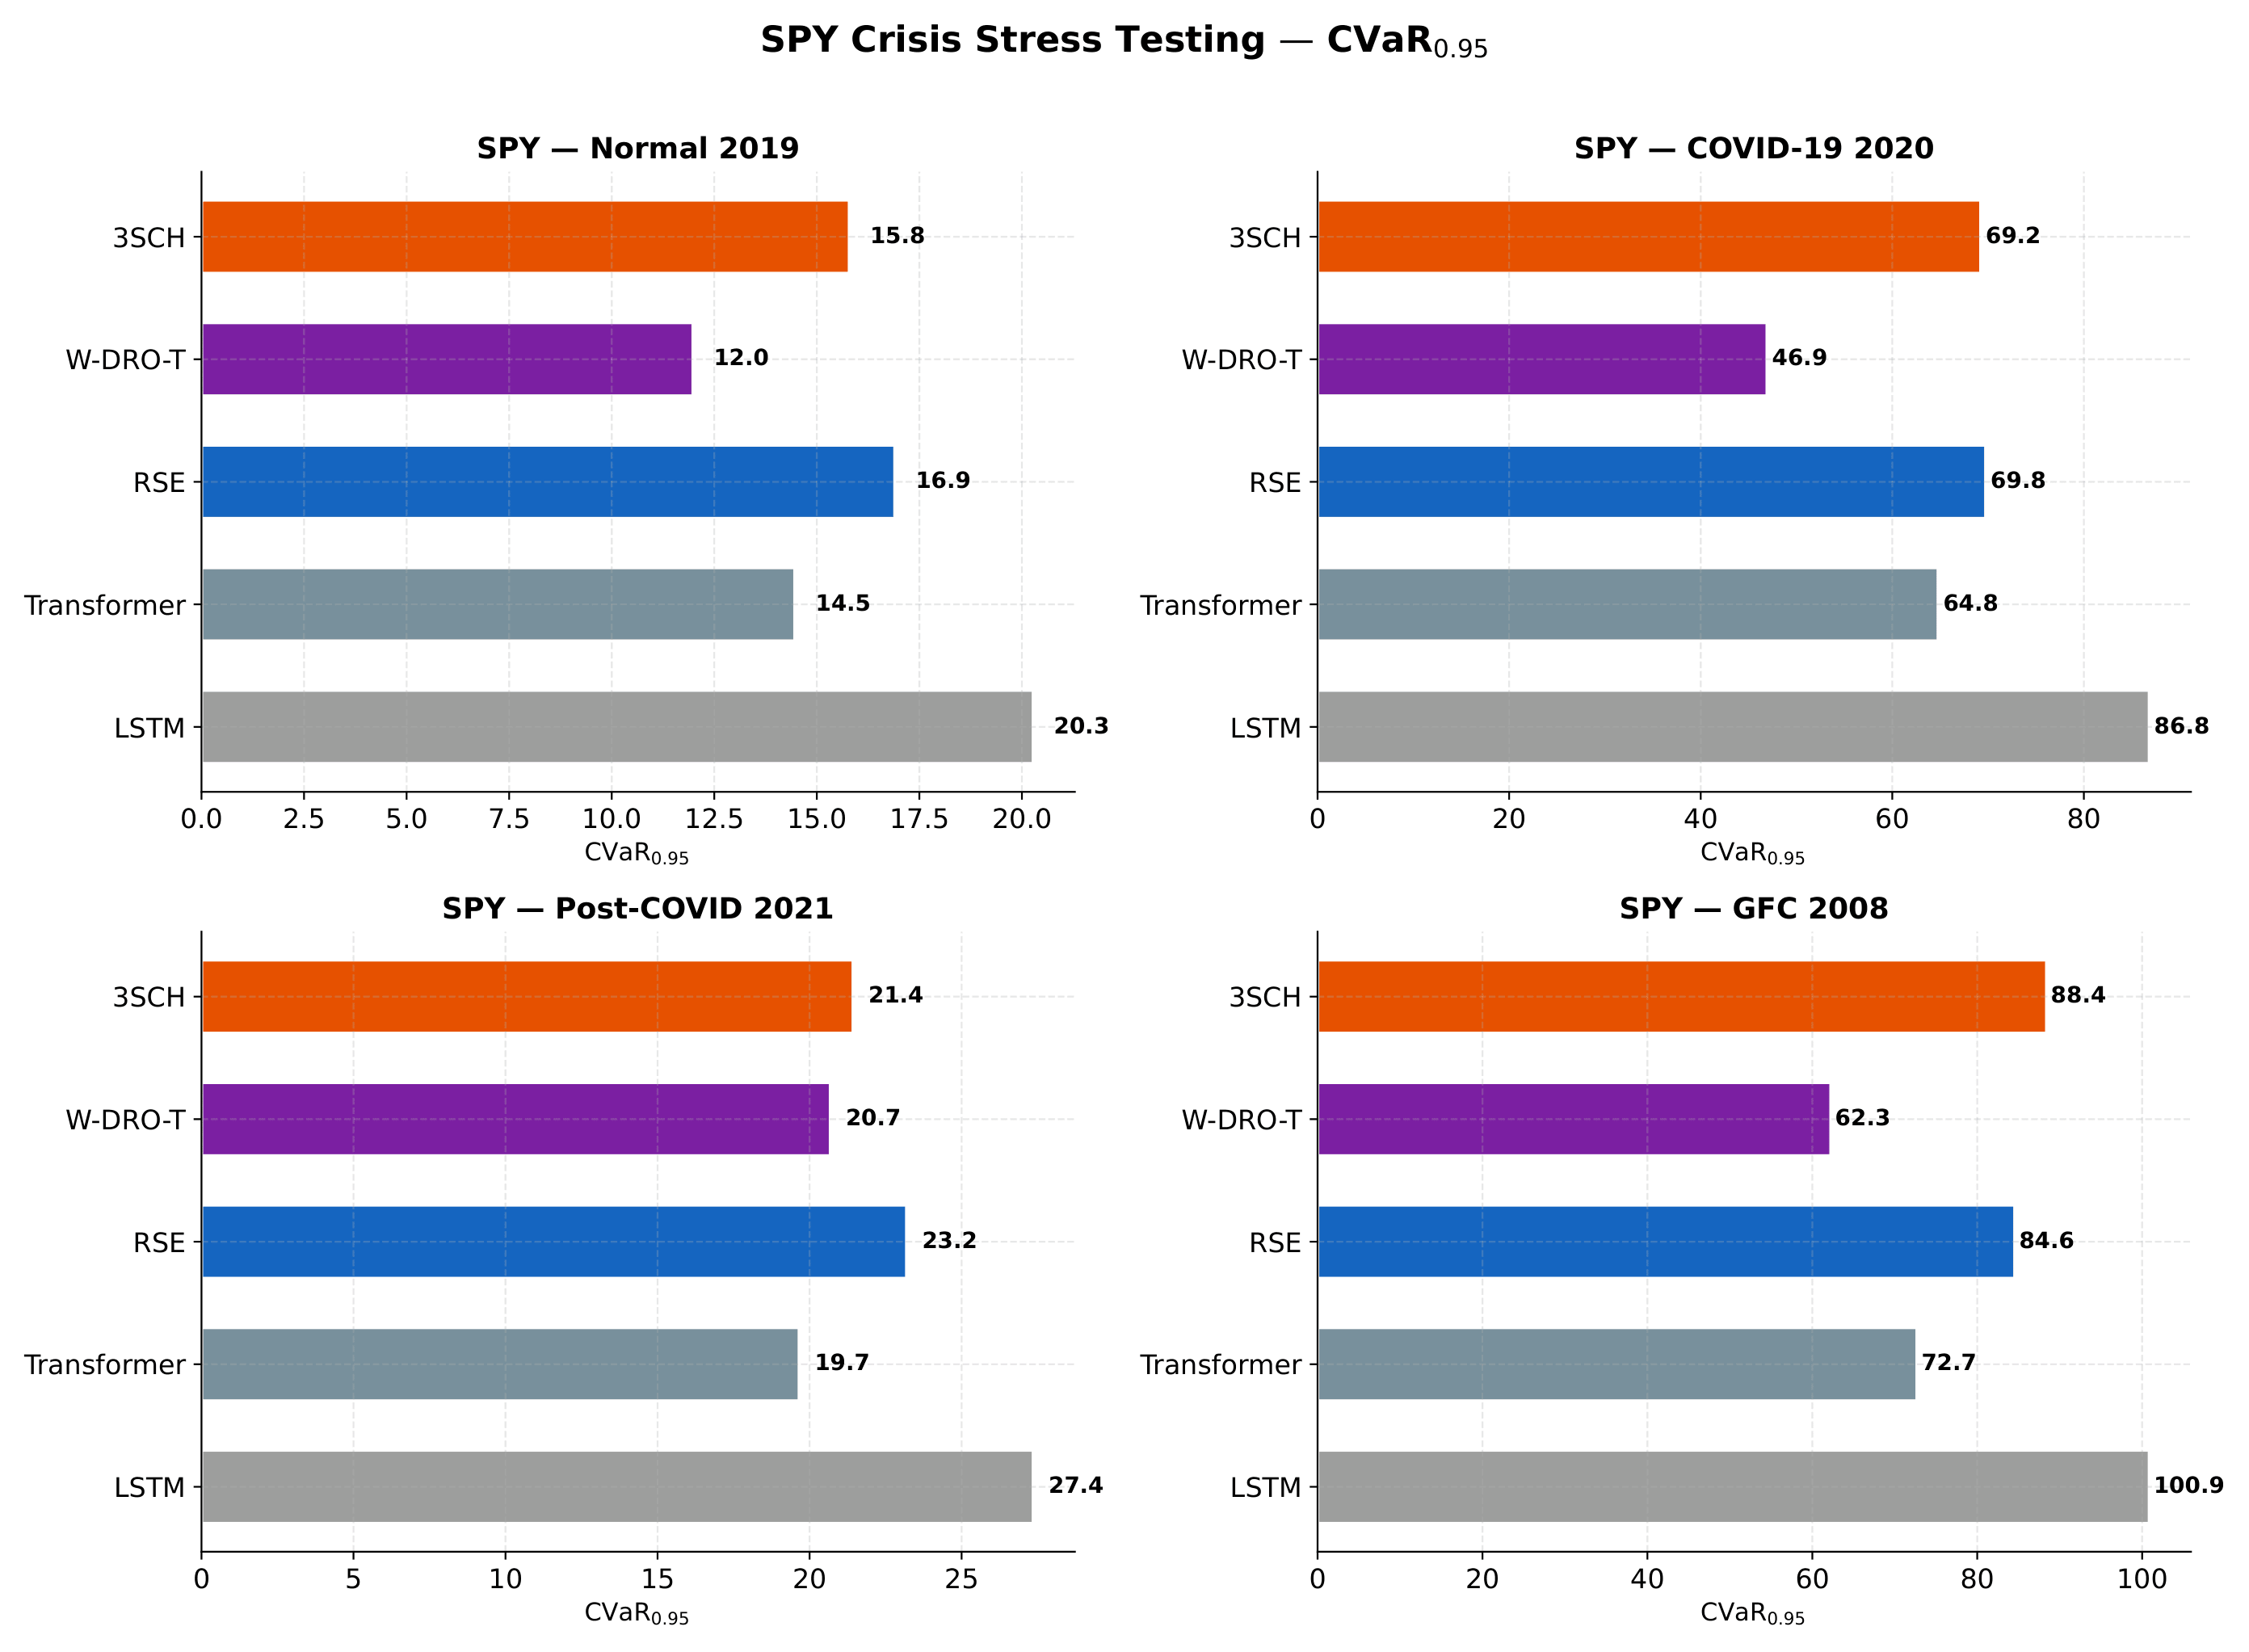
\includegraphics[width=0.92\linewidth]{spy_crisis.png}
\end{center}
\vspace{-4pt}
{\small\color{NavyPri}\textbf{Figure:} SPY crisis stress testing ---
CVaR$_{95}$ across market regimes.}

\bigskip
\textbf{\color{AccWarm}NIFTY\,50 (India, $\sim$18\,bps cost)}

\medskip
{\normalsize
\begin{tabular}{@{}l c c c@{}}
\toprule
\textbf{Model} & \textbf{Normal} & \textbf{COVID-19} & \textbf{GFC-2008} \\
\cmidrule(r){1-1}\cmidrule(lr){2-2}\cmidrule(lr){3-3}\cmidrule(l){4-4}
\textbf{3SCH}  & \textbf{622.26} & 1870.47 & 2499.29 \\
Transformer     & 641.71          & \textbf{1644.19} & 2316.61 \\
W-DRO-T         & 680.34          & 1819.60 & \textbf{2349.58} \\
RSE             & 660.13          & 1758.43 & 2450.91 \\
LSTM            & 627.50          & 1830.28 & 2580.44 \\
\bottomrule
\end{tabular}}

\medskip
{\small 3SCH wins NIFTY normal (lowest cost at 18\,bps);
Transformer wins COVID; W-DRO-T wins GFC.
High friction costs penalise active trading.}
}

%% ── SECTION 6: Economic, Regulatory & Governance ─────────────────
\column{0.48}
\block{\secnum{6}\;\; Economic, Regulatory \& Governance Implications}{
\color{TextBody}

\textbf{\color{NavyPri}Capital requirement analysis (Basel III/IV FRTB)}

\smallskip
$\mathrm{Capital} = m_c \cdot \sqrt{10} \cdot \cvar_{95}
\cdot \mathrm{Notional}/S_0$, \; $m_c = 1.5$.

\medskip
{\normalsize
\begin{tabular}{@{}l r r r@{}}
\toprule
\textbf{Model} & \textbf{Capital (\$/100M)} & \textbf{vs.\ LSTM}
  & \textbf{Std P\&L} \\
\cmidrule(r){1-1}\cmidrule(lr){2-2}\cmidrule(lr){3-3}\cmidrule(l){4-4}
\textbf{W-DRO-T} & \textbf{\$4.79M} & $\mathbf{-41\%}$ & 1.71 \\
Transformer       & \$5.79M          & $-29\%$           & 3.13 \\
3SCH              & \$6.32M          & $-22\%$           & 3.70 \\
RSE               & \$6.76M          & $-17\%$           & 3.57 \\
LSTM              & \$8.11M          & ---               & 5.05 \\
\bottomrule
\end{tabular}}

\medskip
{\small For a \textbf{\$10B desk}: W-DRO-T frees $\sim$\$332M/yr capital;
RSE provides $\sim$\$135M/yr with lower trading costs.}

\bigskip
\begin{center}
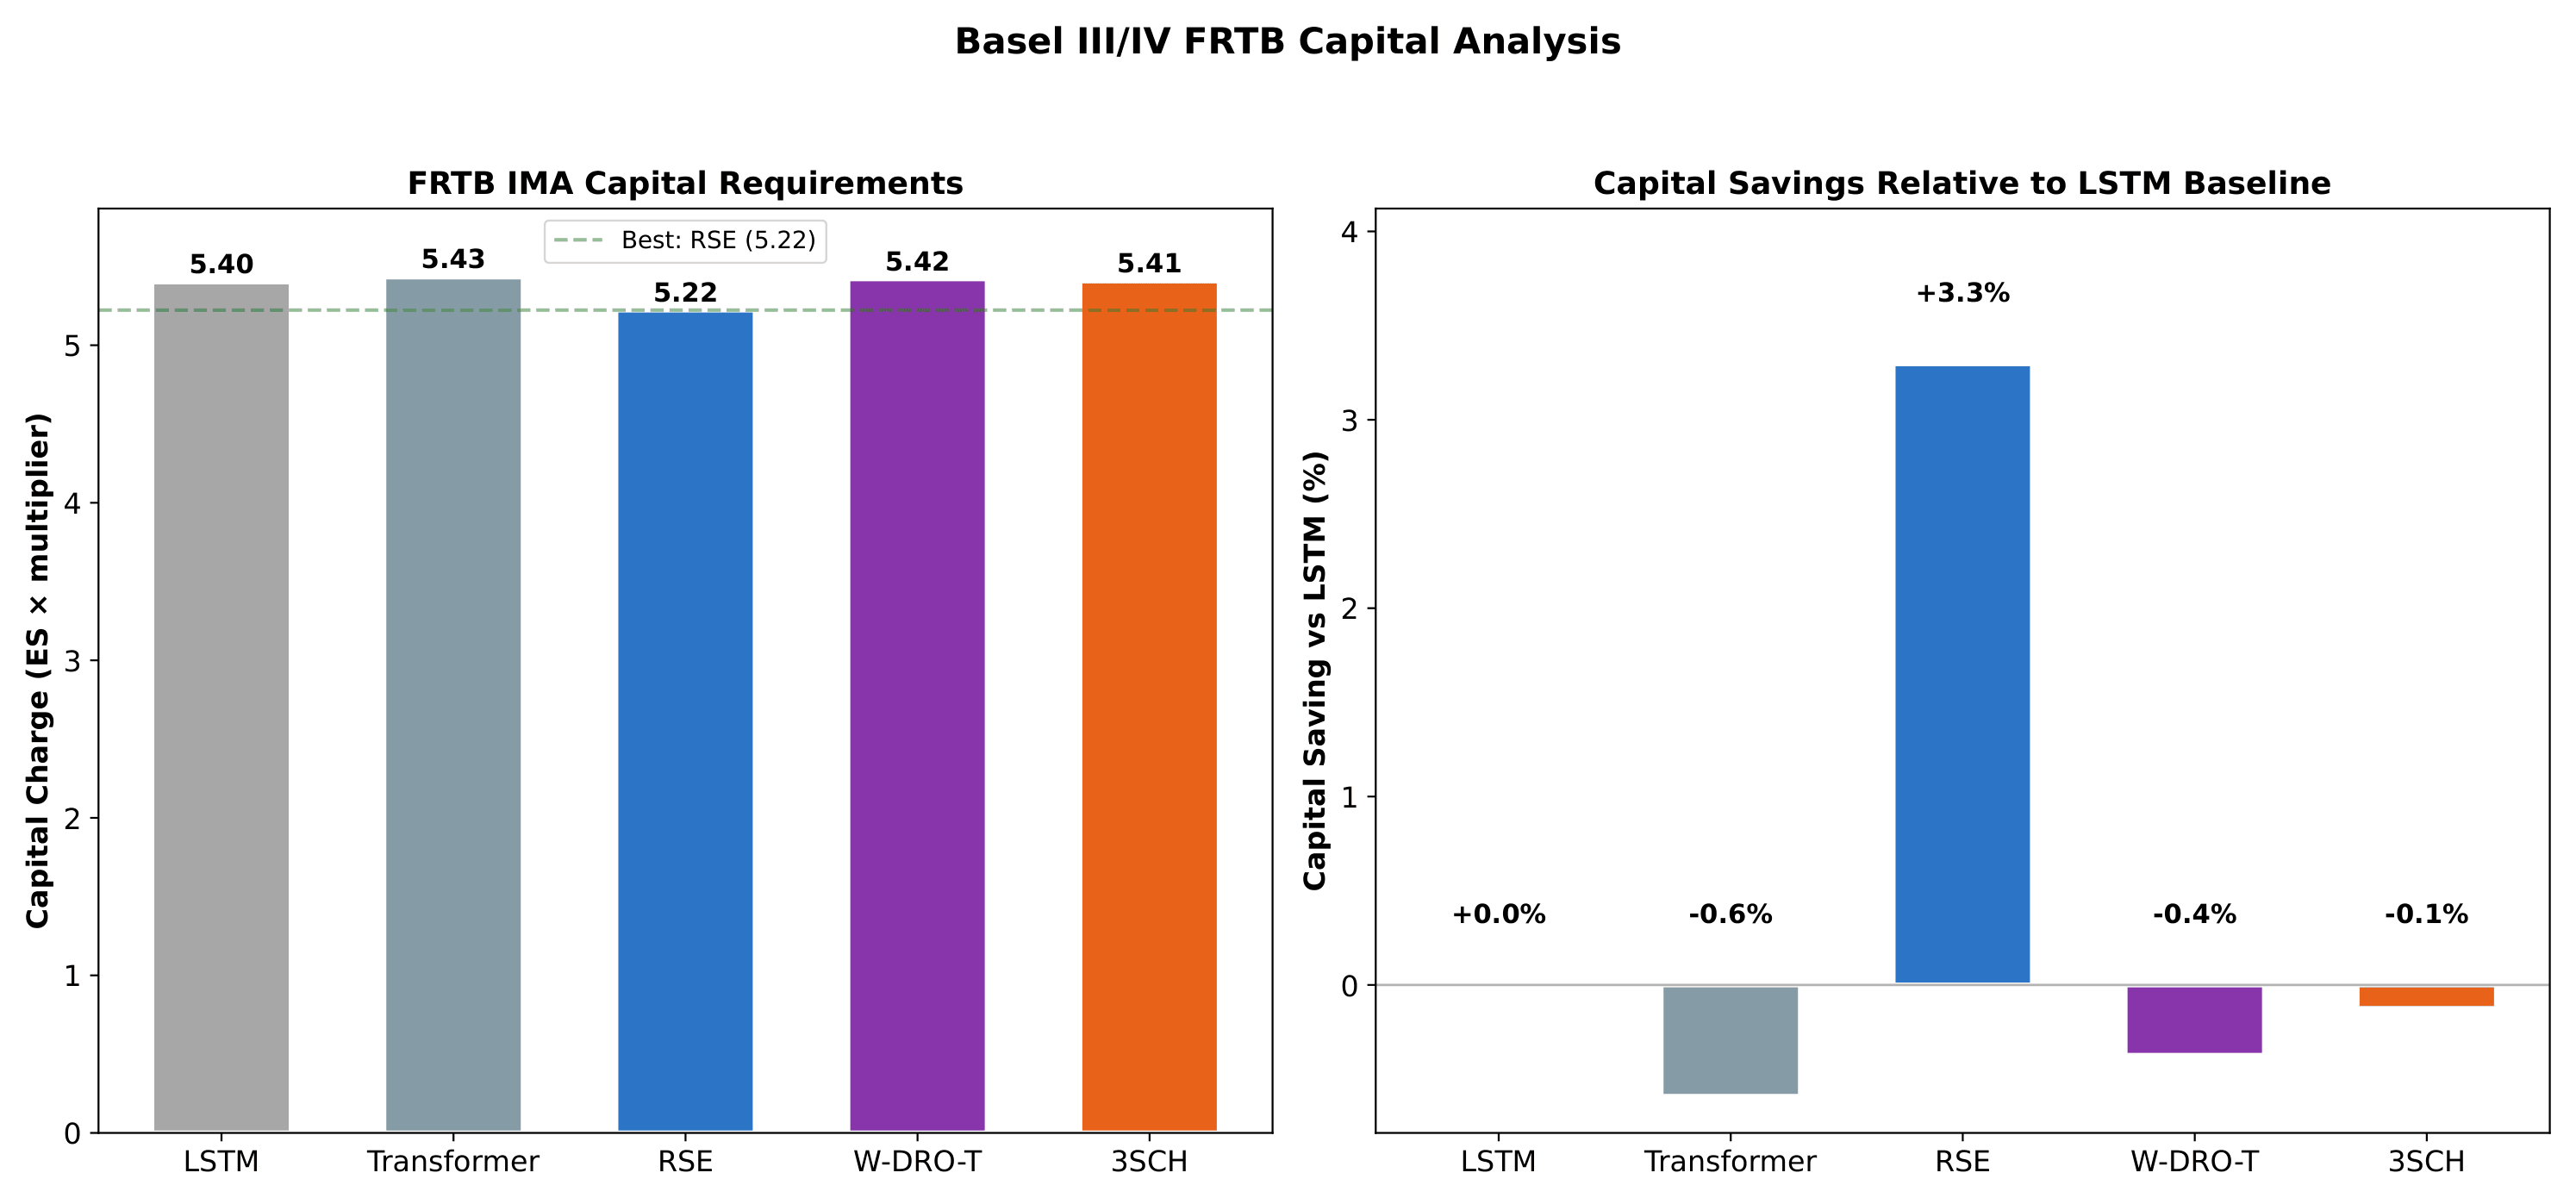
\includegraphics[width=0.92\linewidth]{capital_analysis.png}
\end{center}
\vspace{-4pt}
{\small\color{NavyPri}\textbf{Figure:} Basel III/IV FRTB capital
requirement analysis across models.}

\bigskip
\textbf{\color{NavyPri}Hedge accounting \& regulatory compliance}

\medskip
{\normalsize
\begin{tabular}{@{}l c c c c@{}}
\toprule
\textbf{Model} & \textbf{Offset} & \textbf{$R^2$}
  & \textbf{Std P\&L} & \textbf{Qualifies} \\
\cmidrule(r){1-1}\cmidrule(lr){2-2}\cmidrule(lr){3-3}
\cmidrule(lr){4-4}\cmidrule(l){5-5}
W-DRO-T     & 0.97 & 0.91 & 1.71 & \textcolor{GreenOK}{\ding{51}} \\
RSE         & 0.95 & 0.88 & 3.57 & \textcolor{GreenOK}{\ding{51}} \\
3SCH        & 0.95 & 0.88 & 3.70 & \textcolor{GreenOK}{\ding{51}} \\
LSTM        & 0.94 & 0.87 & 5.05 & \textcolor{GreenOK}{\ding{51}} \\
\bottomrule
\end{tabular}}

\medskip
\begin{itemize}[leftmargin=1em,itemsep=2pt,labelsep=0.3em,topsep=2pt]
\item[\textcolor{GreenOK}{\ding{51}}] \textbf{IAS\,39 / IFRS\,9 /
  Ind-AS\,109:} All models qualify (80--125\% dollar offset)
\item[\textcolor{GreenOK}{\ding{51}}] \textbf{FRTB IMA:} W-DRO-T's low P\&L
  volatility reduces backtesting exceptions
\item[\textcolor{GreenOK}{\ding{51}}] \textbf{SR\,11-7 governance:}
  RSE affinity matrix fully interpretable;
  3SCH = auditable training schedule
\item[\textcolor{GreenOK}{\ding{51}}] \textbf{SEBI compliance:}
  3SCH ideal for Indian markets (minimal complexity)
\end{itemize}

\bigskip
\textbf{\color{NavyPri}Deployment guidance}
\begin{itemize}[leftmargin=1em,itemsep=2pt,labelsep=0.3em,topsep=2pt]
\item[$\triangleright$] \textbf{US markets (3\,bps):} W-DRO-T
  --- best capital savings justify higher trading
\item[$\triangleright$] \textbf{India normal (18\,bps):} 3SCH
  --- lowest CVaR at minimal cost
\item[$\triangleright$] \textbf{Crisis override:} Transformer (NIFTY),
  W-DRO-T (SPY)
\item[$\triangleright$] \textbf{Regime uncertainty:} RSE
  --- best overall CVaR, CV\% = 0.30\%
\end{itemize}
}

\end{columns}

%% ═════════════════════ ROW 4 ═════════════════════════════════════
\begin{columns}

%% ── SECTION 7: Discussion, Limitations & Future ──────────────────
\column{0.48}
\block{\secnum{7}\;\; Discussion, Limitations \& Expected Direction}{
\color{TextBody}

\textbf{\color{NavyPri}When complex models provide value}
\begin{itemize}[leftmargin=1em,itemsep=2pt,labelsep=0.3em,topsep=2pt]
\item[$\triangleright$] \textbf{Crisis environments:} W-DRO-T achieves
  38--46\% CVaR improvement --- justifies complexity
\item[$\triangleright$] \textbf{Capital-constrained desks:}
  41\% savings outweigh operational costs
\item[$\triangleright$] \textbf{Low-cost markets (US, 3\,bps):}
  active strategies are viable
\item[$\triangleright$] \textbf{Regime uncertainty:}
  RSE adapts without retraining; best overall CVaR
\end{itemize}

\medskip
\textbf{\color{AccWarm}When simpler models remain optimal}
\begin{itemize}[leftmargin=1em,itemsep=2pt,labelsep=0.3em,topsep=2pt]
\item[$\triangleright$] \textbf{High-cost markets (India, 18\,bps):}
  active trading penalised; 3SCH optimal
\item[$\triangleright$] \textbf{Regulatory simplicity:}
  LSTM (54K params, 273\,s training) easiest to validate
\item[$\triangleright$] \textbf{Stable conditions:}
  $\sigma \!\approx\! 15\%$ shows small inter-model differentials
\end{itemize}

\bigskip
\textbf{\color{NavyPri}Key limitations}
\begin{itemize}[leftmargin=1em,itemsep=2pt,labelsep=0.3em,topsep=2pt]
\item[$\circ$] Heston model cannot capture jumps, flash crashes,
  or liquidity dry-ups
\item[$\circ$] Single-asset (equity option) --- multi-asset
  portfolio hedging unexplored
\item[$\circ$] Daily OHLCV calibration only (2019--2021);
  intraday microstructure not modelled
\item[$\circ$] W-DRO-T's MATH SDPA requirement limits GPU acceleration
\item[$\circ$] Manual $\varepsilon$ selection; adaptive radius could improve
\end{itemize}

\bigskip
\textbf{\color{SoftBlue}Expected future directions}

\begin{center}
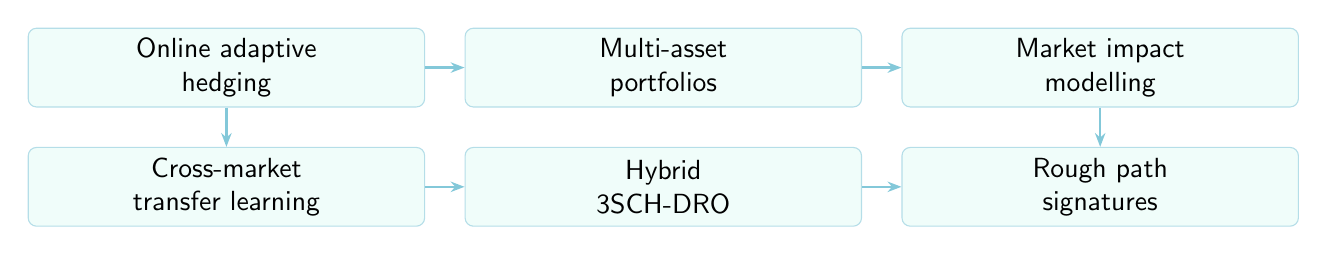
\begin{tikzpicture}[
  dir/.style={rectangle,rounded corners=3pt,draw=SoftBlue!30,
              fill=LightBG,minimum height=10mm,text width=4.8cm,
              text centered,font=\normalsize},
  arr/.style={-{Stealth[length=5pt]},thick,SoftBlue!50}]
\node[dir] (d1) {Online adaptive\\hedging};
\node[dir,right=5mm of d1] (d2) {Multi-asset\\portfolios};
\node[dir,right=5mm of d2] (d3) {Market impact\\modelling};
\node[dir,below=5mm of d1] (d4) {Cross-market\\transfer learning};
\node[dir,below=5mm of d2] (d5) {Hybrid\\3SCH-DRO};
\node[dir,below=5mm of d3] (d6) {Rough path\\signatures};
\draw[arr] (d1)--(d2); \draw[arr] (d2)--(d3);
\draw[arr] (d4)--(d5); \draw[arr] (d5)--(d6);
\draw[arr] (d1)--(d4); \draw[arr] (d3)--(d6);
\end{tikzpicture}
\end{center}
}

%% ── SECTION 8: References, Acknowledgement, Contact, QR ─────────
\column{0.48}
\block{\secnum{8}\;\; References}{
\color{TextBody}
{\small
\begin{enumerate}[leftmargin=1.8em,itemsep=1pt,topsep=2pt,label={[\arabic*]}]
\item Heston, S.\,L.\ (1993).
  A Closed-Form Solution for Options with Stochastic Volatility with
  Applications to Bond and Currency Options.
  \textit{Rev.\ Financial Studies}, 6(2), 327--343.
\item Buehler, H., Gonon, L., Teichmann, J., \& Wood, B.\ (2019).
  Deep Hedging. \textit{Quantitative Finance}, 19(8), 1271--1291.
\item Rockafellar, R.\,T.\ \& Uryasev, S.\ (2000).
  Optimization of Conditional Value-at-Risk.
  \textit{J.\ Risk}, 2(3), 21--41.
\item Blanchet, J.\ \& Murthy, K.\ (2019).
  Quantifying Distributional Model Risk via Optimal Transport.
  \textit{Math.\ Operations Research}, 44(2), 565--600.
\item Vaswani, A.\ et al.\ (2017).
  Attention Is All You Need.
  \textit{Adv.\ Neural Inf.\ Proc.\ Sys.\ (NeurIPS)}, 30.
\item Bengio, Y., Louradour, J., Collobert, R., \& Weston, J.\ (2009).
  Curriculum Learning.
  \textit{Proc.\ ICML}, 41--48.
\item Dietterich, T.\,G.\ (2000).
  Ensemble Methods in Machine Learning.
  \textit{Proc.\ MCS}, LNCS 1857, 1--15.
\item Esfahani, P.\,M.\ \& Kuhn, D.\ (2018).
  Data-driven Distributionally Robust Optimization Using the
  Wasserstein Metric. \textit{Math.\ Programming}, 171, 115--166.
\item Lyons, T.\,J.\ (1998).
  Differential Equations Driven by Rough Signals.
  \textit{Rev.\ Mat.\ Iberoamericana}, 14(2), 215--310.
\item Kozyra, J.\ (2019).
  Deep Hedging with Curriculum Learning.
  MSc Thesis, University of Oxford.
\item F{\"o}llmer, H.\ \& Schied, A.\ (2002).
  Convex Measures of Risk and Trading Constraints.
  \textit{Finance \& Stochastics}, 6(4), 429--447.
\item L{\"u}tkebohmert, E.\ \& Sester, J.\ (2021).
  Robust Deep Hedging.
  \textit{SSRN Working Paper}.
\end{enumerate}
}

\bigskip
\textbf{\large\color{NavyPri}Acknowledgement}

\medskip
{\normalsize
The author gratefully acknowledges the guidance and supervision of
\textbf{Prof.\ Aditi Gangopadhyay}, the esteemed committee panel,
and the support of the \textbf{Department of Mathematics, IIT Roorkee},
during the course of this thesis work.}

\bigskip
\textbf{\large\color{NavyPri}Contact}

\medskip
\begin{minipage}[t]{0.55\linewidth}
{\normalsize
\textbf{Email:} \texttt{p\_kailasiya@ma.iitr.ac.in}\\[4pt]
\textbf{Mobile:} +91-7000320877\\[4pt]
\textbf{Dept.:} Mathematics, IIT Roorkee\\[4pt]
\textbf{Programme:} BS-MS, Math \& Computing}
\end{minipage}
\hfill
\begin{minipage}[t]{0.40\linewidth}
\centering
\begin{tikzpicture}
\node[inner sep=0pt] (gh) {
\includegraphics[width=4.5cm]{github_qr.png}};
\node[below=3mm of gh,font=\small\bfseries\color{NavyPri}] {GitHub};
\node[inner sep=0pt,right=10mm of gh] (li)
  {
\includegraphics[width=4.5cm]{linkedin_qr.png}};
\node[below=3mm of li,font=\small\bfseries\color{NavyPri}] {LinkedIn};
\end{tikzpicture}
\end{minipage}
}

\end{columns}

\end{document}
